% Options for packages loaded elsewhere
\PassOptionsToPackage{unicode}{hyperref}
\PassOptionsToPackage{hyphens}{url}
\PassOptionsToPackage{dvipsnames,svgnames,x11names}{xcolor}
%
\documentclass[
  letterpaper,
  DIV=11,
  numbers=noendperiod]{scrartcl}

\usepackage{amsmath,amssymb}
\usepackage{iftex}
\ifPDFTeX
  \usepackage[T1]{fontenc}
  \usepackage[utf8]{inputenc}
  \usepackage{textcomp} % provide euro and other symbols
\else % if luatex or xetex
  \usepackage{unicode-math}
  \defaultfontfeatures{Scale=MatchLowercase}
  \defaultfontfeatures[\rmfamily]{Ligatures=TeX,Scale=1}
\fi
\usepackage{lmodern}
\ifPDFTeX\else  
    % xetex/luatex font selection
\fi
% Use upquote if available, for straight quotes in verbatim environments
\IfFileExists{upquote.sty}{\usepackage{upquote}}{}
\IfFileExists{microtype.sty}{% use microtype if available
  \usepackage[]{microtype}
  \UseMicrotypeSet[protrusion]{basicmath} % disable protrusion for tt fonts
}{}
\makeatletter
\@ifundefined{KOMAClassName}{% if non-KOMA class
  \IfFileExists{parskip.sty}{%
    \usepackage{parskip}
  }{% else
    \setlength{\parindent}{0pt}
    \setlength{\parskip}{6pt plus 2pt minus 1pt}}
}{% if KOMA class
  \KOMAoptions{parskip=half}}
\makeatother
\usepackage{xcolor}
\ifLuaTeX
  \usepackage{luacolor}
  \usepackage[soul]{lua-ul}
\else
  \usepackage{soul}
  
\fi
\setlength{\emergencystretch}{3em} % prevent overfull lines
\setcounter{secnumdepth}{-\maxdimen} % remove section numbering
% Make \paragraph and \subparagraph free-standing
\ifx\paragraph\undefined\else
  \let\oldparagraph\paragraph
  \renewcommand{\paragraph}[1]{\oldparagraph{#1}\mbox{}}
\fi
\ifx\subparagraph\undefined\else
  \let\oldsubparagraph\subparagraph
  \renewcommand{\subparagraph}[1]{\oldsubparagraph{#1}\mbox{}}
\fi


\providecommand{\tightlist}{%
  \setlength{\itemsep}{0pt}\setlength{\parskip}{0pt}}\usepackage{longtable,booktabs,array}
\usepackage{calc} % for calculating minipage widths
% Correct order of tables after \paragraph or \subparagraph
\usepackage{etoolbox}
\makeatletter
\patchcmd\longtable{\par}{\if@noskipsec\mbox{}\fi\par}{}{}
\makeatother
% Allow footnotes in longtable head/foot
\IfFileExists{footnotehyper.sty}{\usepackage{footnotehyper}}{\usepackage{footnote}}
\makesavenoteenv{longtable}
\usepackage{graphicx}
\makeatletter
\def\maxwidth{\ifdim\Gin@nat@width>\linewidth\linewidth\else\Gin@nat@width\fi}
\def\maxheight{\ifdim\Gin@nat@height>\textheight\textheight\else\Gin@nat@height\fi}
\makeatother
% Scale images if necessary, so that they will not overflow the page
% margins by default, and it is still possible to overwrite the defaults
% using explicit options in \includegraphics[width, height, ...]{}
\setkeys{Gin}{width=\maxwidth,height=\maxheight,keepaspectratio}
% Set default figure placement to htbp
\makeatletter
\def\fps@figure{htbp}
\makeatother

\KOMAoption{captions}{tableheading}
\makeatletter
\@ifpackageloaded{caption}{}{\usepackage{caption}}
\AtBeginDocument{%
\ifdefined\contentsname
  \renewcommand*\contentsname{Table of contents}
\else
  \newcommand\contentsname{Table of contents}
\fi
\ifdefined\listfigurename
  \renewcommand*\listfigurename{List of Figures}
\else
  \newcommand\listfigurename{List of Figures}
\fi
\ifdefined\listtablename
  \renewcommand*\listtablename{List of Tables}
\else
  \newcommand\listtablename{List of Tables}
\fi
\ifdefined\figurename
  \renewcommand*\figurename{Figure}
\else
  \newcommand\figurename{Figure}
\fi
\ifdefined\tablename
  \renewcommand*\tablename{Table}
\else
  \newcommand\tablename{Table}
\fi
}
\@ifpackageloaded{float}{}{\usepackage{float}}
\floatstyle{ruled}
\@ifundefined{c@chapter}{\newfloat{codelisting}{h}{lop}}{\newfloat{codelisting}{h}{lop}[chapter]}
\floatname{codelisting}{Listing}
\newcommand*\listoflistings{\listof{codelisting}{List of Listings}}
\makeatother
\makeatletter
\makeatother
\makeatletter
\@ifpackageloaded{caption}{}{\usepackage{caption}}
\@ifpackageloaded{subcaption}{}{\usepackage{subcaption}}
\makeatother
\ifLuaTeX
  \usepackage{selnolig}  % disable illegal ligatures
\fi
\usepackage{bookmark}

\IfFileExists{xurl.sty}{\usepackage{xurl}}{} % add URL line breaks if available
\urlstyle{same} % disable monospaced font for URLs
\hypersetup{
  colorlinks=true,
  linkcolor={blue},
  filecolor={Maroon},
  citecolor={Blue},
  urlcolor={Blue},
  pdfcreator={LaTeX via pandoc}}

\author{}
\date{}

\begin{document}

\newpage

\begin{verbatim}
Warning: Using `size` aesthetic for lines was deprecated in ggplot2 3.4.0.
i Please use `linewidth` instead.
\end{verbatim}

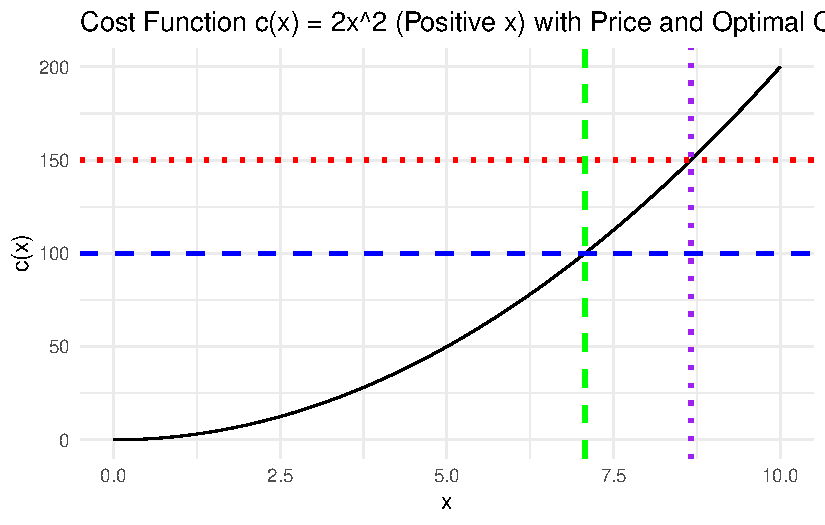
\includegraphics{arbeidskrav_files/figure-pdf/unnamed-chunk-2-1.pdf}

\subsubsection{Obligatorisk
innleveringsoppgaver}\label{obligatorisk-innleveringsoppgaver}

\begin{itemize}
\tightlist
\item
  Innleveringsfrist: \textbf{31.3}.

  \begin{itemize}
  \tightlist
  \item
    \href{https://hiof.instructure.com/courses/8577/assignments/38559}{Canvas}
  \end{itemize}
\item
  Versjon 1.1
\item
  Kan jobbe alene, eller levere som gruppe (bestemmer selv antallet, men
  utbytte av arbeidskravet vil nok være større ved en mindre gruppe)
\end{itemize}

\subsection{Oppgave 1: Generell
forståelse}\label{oppgave-1-generell-forstuxe5else}

I. Er følgende påstander riktig eller gale? Begrunn svaret ditt med
økonomisk teori.

\begin{enumerate}
\def\labelenumi{\alph{enumi}.}
\tightlist
\item
  Økonomi handler først og fremst om penger.

  Galt: Handler først og fremst om forvaltningen av knappe ressurser for
  å dekke menneskelige behov.
\item
  Følgende produktfunksjon er konkav:
  \(X(N)=N^{\alpha} \text{ der } 0<\alpha<1.\)

  Riktig: Siden ved bruk av arbeidskraft vil
  \(X'(N)=\alpha N^{\alpha-1} >0\) og
  \(X''(N)=(\alpha-1)\alpha N^{\alpha-2} <0\)
\item
  Grenseinntekten til en bedrift viser hvor mye mer bedriften kan
  produsere dersom inntekten stiger med 1 krone.

  Galt: Grenseinntekten viser inntektsendring som følge av at
  produksjonen øker med én enhet.
\item
  Anta Mona sin MSB = 4. Det betyr at Mona er villig til å gi bort 4
  enheter av gode 2 for én ekstra enhet av gode 1.

  Riktig: MSB forteller oss at dersom vi øker det som står på x-aksen
  (gode 1) med én enhet, hvor mye vi må oppgi av det gode som står på
  y-aksen (gode 2) gitt at vi skal være på samme nyttenivå. I dette
  tilfelle dreier det seg om 4 enheter.
\end{enumerate}

II: Forklar følgende begreper:

\begin{enumerate}
\def\labelenumi{\alph{enumi}.}
\tightlist
\item
  Nyttefunksjon

  En funksjon som for enhver godekombinasjon gir oss den samlede nytten
  ved å konsumerer denne godekombinasjonen. Gitt en ordinal
  nyttefunksjon, vil den samlede nytten være gitt ved et tall som
  rangerer godekombinasjonene, dvs. høyere tall desto bedre rangering.
\item
  Grensenytte

  Endring i nytte av å motta én ekstra enhet av et gode.
\item
  Marginal substitusjonsbrøk (MSB)

  Gitt som forholdet mellom grensenytten av de to godene. Vi kan
  uttrykke (\(\frac{U'(X_{1})}{U'(X_{2})}\)), og verdien som fremkommer
  forteller hvor mange enheter av gode \(X_{2}\) man er villig til å
  oppgi for å oppnå én enhet ekstra av gode \(X_{1}\).
\item
  For konsumenten, sammenhengen mellom den marginale betalingsviligheten
  (MBV) og betalingsvilligheten (BV)

  Betalingsvilligheten (BV) for et vist antall goder X er gitt som
  summen av den marginale betalingsviligheten (MBV) til hvert enkelt
  gode opp til og med X.
\item
  For bedriften, sammenhengen mellom den marginale grensekostnaden (GK)
  og de variable kostnadene (VK)

  De variable kostnadene for et gitt kvantum x er gitt som summen av de
  marginale grensekostnaden (MG) for alle kvantum opp til og med X.
\end{enumerate}

\begin{enumerate}
\def\labelenumi{\Roman{enumi}.}
\setcounter{enumi}{2}
\tightlist
\item
  Ta utgangspunkt i en fallende etterspørselskurve i et pris-mengde
  diagram.
\end{enumerate}

\begin{enumerate}
\def\labelenumi{\alph{enumi}.}
\tightlist
\item
  Vis hvordan etterspørselskurven påvirkes av økt inntekt blant
  konsumentene dersom godet er normalt, og mindreverdig.

  Ved normalt gode, etterspørselskurven skifter til høyre. Ved
  mindreverdig gode, skifter til venstre.
\item
  Vis hvordan etterspørselskurven påvirkes av økt pris på en alternativ
  vare.

  Ved økt pris på alternativ vare, etterspørselskurven skifter til
  høyre.
\end{enumerate}

\subsection{Oppgave 2: Produksjonsteori på kort
sikt}\label{oppgave-2-produksjonsteori-puxe5-kort-sikt}

Bedriften Cambå produserer handlevogner hvor kostnadsfunksjonen gitt ved
\(C = 2 x^{2}\). Produktprisen er gitt ved \(100\) kroner.

\begin{enumerate}
\def\labelenumi{\alph{enumi})}
\tightlist
\item
  Gi en forklaring på egenskapene til Cambå sine grensekostnader.

  Siden vi har at \(C'(x)=4x^{2-1}=4 x>0\) og \(C''(X)=4>0\) kan vi si
  at grensekostnaden er positive og stigende. Dvs. desto flere
  produserte enheter, desto høyere grensekostnader, og hvor
  kostnadsøkningen som kommer som en følge av den siste enheten vil være
  større enn de foregående enhetene.
\item
  Finn betingelsen (førsteordens-betingelsen) som maksimerer
  fortjenesten til bedriften. Gi deretter en økonomisk tolkning av denne
  tilpasningsbetingelsen.

  Uttrykket for fortjensten (F) er gitt ved \[
  F=pX-C(x)=100x-2x^2
  \] Ved å maksimere dette uttrykket mhp. \(x\), finner vi at
  betingelsen (førsteordens) for antall produserte enheter som gjør
  fortjenesten størst mulig:

  \begin{aligned}
  100 - 4 x = 0 \Leftrightarrow 100=4x
  \end{aligned}

  Tolkning: produksjonen settes slik at grensekostnaden er lik
  produktprisen. Dette er optimalt, siden dersom produkprisen er høyere
  (lavere) enn grensekostnaden vil bedriften øke sin fortjeneste ved øke
  (redusere) sin produksjon.
\item
  Hvor mange enheter vil Cambå måtte produsere gitt at bedriften har som
  mål å maksimere sin fortjeneste?

  Dersom vi løser førsteordensbetingelsen mhp. på \(x\) finner vi at
  dette produksjonsvolumet er gitt ved \[
  4x=100 \Rightarrow x = \frac{100}{4}=25
  \]
\item
  Hva blir fortjenesten til bedriften i dette tilfellet?

  Fortjenesten vil derfor her være gitt ved

  \begin{aligned}
  \text{F} = 100\cdot 25 − 2\cdot 25^2 = 2500 − 1250 = 1250
  \end{aligned}
\item
  Vis ved bruk av en figur og forklar hva som skjer med tilbudet til
  bedriften i produktmarkedet dersom prisen øker.

  Dersom produktprisen øker, vil grensekostnaden i utgangspunktet være
  lavere enn produktprisen. Det vil gjøre det lønnsomt for bedriften å
  øke tilbudet helt inntil betingelsen om at grensekostnad skal være
  like produktpris er oppfylt.
\item
  Vi lar bruken av arbeidskraft være representert ved N. Vis at
  produksjonsfunksjonen\\
  \(x = N^{0.5}\) gir opphav til de variable kostnadene som er lik
  \(2 x^{2}\) gitt at lønnskostnaden per arbeider er lik \st{1} 2
  kroner.

  \begin{aligned}
  x=N^{0.5} \\
  x^2=N \\
  N=x^2 \\
  \end{aligned}

  Hvor faktorutlegget vil være lik de variable kostnadene som vil være
  git ved

  \begin{aligned}
  C_v=wN=2X^2 
  \end{aligned}
\end{enumerate}

\subsection{Oppgave 3: Konsumentteori}\label{oppgave-3-konsumentteori}

Anta en konsument med følgende nyttefunksjon: \begin{equation}
U(x_{1}, x_{2}) = 7x_{1}x_{2}
\end{equation} Konsumentens budsjettbetingelse er gitt ved
\(p_{1}x_{1} + p_{2}x_{2} = R\), der \(R = 600\), \(p_{1} = 2\) og
\(p_{2} = 4\).

\begin{enumerate}
\def\labelenumi{\alph{enumi}.}
\tightlist
\item
  Finn optimalt konsum av de to godene.

  Førsteordensbetinigelsene fra Lagrange-metode gir oss et system
  bestående av to ligninger:

  \begin{aligned}
  MSB=\frac{p_1}{p_2}\\
  p_{1}x_{1} + p_{2}x_{2} = R
  \end{aligned}

  Ved å ta utgangspunkt i informasjonen gitt i oppgaven får vi

  \begin{aligned}
  \frac{x_2}{x_1}=\frac{2}{4}=\frac{1}{2}\\
  2x_{1} + 4x_{2} = 600
  \end{aligned}

  Løser det første uttrykket mph \(4x_2=2x_1\) og setter dette inn i
  budsjettbetingelsen gir oss

  \begin{aligned}
  2x_1 + 2x_1 = 600 \\
  x_1(2+2) = 600 \\
  x_1 = 600/4 =  150
  \end{aligned}

  Setter denne løsningen tilbake i budsjettbetingelsen for å finne

  \begin{aligned}
  2\cdot 150 + 4x_2 = 600 \\
  4x_2 = 600 - 300 \\
  x_2 = 300/4 = 75 \\
  (\text{Kontroll:} \frac{x_2}{x_1}=\frac{75}{150}=\frac{1}{2})  
  \end{aligned}
\item
  Anta at prisen på gode 1 øker til 3. Hva blir etterspørselen etter
  gode 1 nå?

  Løser det første uttrykket mph \(4x_2=3x_1\) og setter dette inn i
  budsjettbetingelsen gir oss

  \begin{aligned}
  3x_1 + 3x_1 = 600 \\
  x_1(3+3) = 600 \\
  x_1 = 600/6 =  100\\
  \end{aligned}
\item
  Regn ut egenpriselastisiteten basert på \%-vis endring i etterspørsel
  og pris. Kategoriser elastisiteten.

  \begin{aligned}
  \frac{\Delta x_{1}}{x_{1}}/\frac{\Delta p_{1}}{p_{1}}=\frac{\Delta (100-150)}{150}/\frac{\Delta (3-2)}{2}=-0.33/0.5=-0.66
  \end{aligned}

  Siden verdien ligger i intervallet mellom -1 og 0 \(\rightarrow\)
  godet er prisuelastisk.
\end{enumerate}

\subsection{Oppgave 4: Markedsteori: Fullkommen konkurranse med og uten
avgift}\label{oppgave-4-markedsteori-fullkommen-konkurranse-med-og-uten-avgift}

Vi ser på et marked under fullkommen konkurranse. Etterspørselen er gitt
ved (den marginale betalingsvillighet) \(P = 24 – 2X\) og tilbudet
(grensekostnaden) som \(P = 4X\).

\begin{enumerate}
\def\labelenumi{\alph{enumi})}
\tightlist
\item
  Finn likevektspris og omsatt kvantum. Vis tilpasningen grafisk.

  Vi starter med omsatt kvantum. I fullkommen vil løsningen være
  karakterisert ved at MBV=GK, det gir oss

  \begin{aligned}
  24-2x=4x \\
  6x   =24 \\
  x^{FK}=x =\frac{24}{6} = 4
  \end{aligned}

  Setter vi dette kvantumet inn i enten etterspørs- eller tilbudskurven
  vil vi finne produktprisen

  \begin{aligned}
  MBV: P = 24-2\cdot 4=16 \\
  (GK: P = 4\cdot 4= 16)
  \end{aligned}
\item
  Regn ut konsumentoverskuddet (KO), produsentoverskuddet (PO) og
  samfunnsøkonomisk overskudd (SO).

  Konsumentoverskuddet er gitt ved arealet til trekanten

  \begin{aligned}
  KO = (4-0)\cdot(24-16)/2 = 16
  \end{aligned}

  Mens produsentoverskudet er gitt ved

  \begin{aligned}
  PO = (4-0)(16)/2 = 32
  \end{aligned}

  Samfunnsøkonomisk overskudd blir derfor

  \begin{aligned}
  SO = PO+KO =32+16= 48
  \end{aligned}
\item
  For å skaffe inntekter til statskassen, innføres en skatt på 6 kroner
  per produsert enhet. Regn ut \(P_K\) (pris til konsument), \(P_P\)
  (pris til produsent) og omsatt kvantum \(X\).

  Skatt per enhet gjør at tilbudskurven kan skrives som

  \begin{aligned}
  P = 4x + 6 \\
  24-2x=4x+6 \\
  6x   =18 \\
  x = 3
  \end{aligned}

  Prisen til konsument blir derfor

  \begin{aligned}
  P_k = 24 - 2\cdot 3 = 18
  \end{aligned}

  Mens pris til produsent blir

  \begin{aligned}
  P_p=4\cdot3 = 12
  \end{aligned}
\item
  Hva blir KO, PO og SO denne gangen? Vi antar her at skatteinntekten
  inngår i det samfunnsøkonomiske overskuddet.

  Konsument- , produsentoverskudd og samfunnsøkonomisk overskudd er nå
  gitt ved

  \begin{aligned}
  KO = \frac{(3\cdot (24-18))}{2}  = 9\\
  PO = (3\cdot (12-0))/2 = 18\\
  SI = 3\cdot (18-12)= 18 \\
  SO (\text{med tilbakebetaling av SI til KO og PO})= 9+18+18=45
  \end{aligned}
\item
  Regn ut effektivitetstapet og illustrer denne tilpasningen ved hjelp
  av en figur.

  \begin{equation}
  DT = \frac{(4-3)\cdot (18-12)}{2}=3
  \end{equation}
\item
  Vil de samfunnsøkonomiske konsekvensene av avgiften bli påvirket av
  etterspørselens og tilbudets prisfølsomhet (priselastisitet)? Begrunn
  svaret.

  Essensen med stykkavgiften på 6 kroner er at den medfører et
  effektivitetstap som følge av at den skaper en kile mellom den prisen
  som kundene betaler og den pris produsentene mottar. Generelt vil det
  være slik at desto mer priselastisk etterspørselen og tilbudet er,
  desto større vil effektivitetstapet være.
\end{enumerate}

\href{https://github.com/joernih/SFB10816Mikrooekonomi/blob/main/utskrifter/Arbeidskrav_2024_V.pdf}{Trykk
her for pdf-versjon}

Vis svar (figurer vil bli lagt til snart)



\end{document}
